%compile with pdflatex on papeeria

\documentclass[a4paper,12pt]{article}
\usepackage{fancyhdr}
%\usepackage{fancyheadings}
\usepackage[ngerman,german]{babel}
\usepackage{german}
\usepackage[utf8]{inputenc}
%\usepackage[latin1]{inputenc}
\usepackage[active]{srcltx}
%\usepackage{algorithm}
%\usepackage[noend]{algorithmic}
\usepackage{amsmath}
\usepackage{amssymb}
\usepackage{amsthm}
\usepackage{bbm}
\usepackage{enumerate}
\usepackage{graphicx}
\usepackage{ifthen}
\usepackage{listings}
\usepackage{enumitem}
%\usepackage{struktex}
\usepackage{hyperref}
\usepackage{tikz}
\usepackage{float}
\usepackage{subcaption}
\usepackage{array}
\captionsetup{compatibility=false}
\captionsetup[subfigure]{labelformat=empty}

\usepackage{pgfplots}
\usepgfplotslibrary{fillbetween}
%\usetikzlibrary{patterns}
\pgfplotsset{compat=1.15}
\usepackage{mathrsfs}
\usetikzlibrary{arrows}

\pgfplotsset{grid style={dashed,gray}}

\definecolor{kolorwykresu}{rgb}{0.07,0.04,0.56}

\pagenumbering{gobble}

\usepackage{tabularray}
\usepackage{multirow}
\usepackage{booktabs,tabularx}
\renewcommand\tabularxcolumn[1]{m{#1}}% for vertical centering text in X column

\newcolumntype{L}[1]{>{\raggedright\let\newline\\\arraybackslash\hspace{0pt}}m{#1}}
\newcolumntype{C}[1]{>{\centering\let\newline\\\arraybackslash\hspace{0pt}}m{#1}}
\newcolumntype{R}[1]{>{\raggedleft\let\newline\\\arraybackslash\hspace{0pt}}m{#1}}

\newcolumntype{Y}{>{\centering\arraybackslash}X}

%%%%%%%%%%%%%%%%%%%%%%%%%%%%%%%%%%%%%%%%%%%%%%%%%%%%%%
%%%%%%%%%%%%%% EDIT THIS PART %%%%%%%%%%%%%%%%%%%%%%%%
%%%%%%%%%%%%%%%%%%%%%%%%%%%%%%%%%%%%%%%%%%%%%%%%%%%%%%
\newcommand{\Fach}{1. Klausur aus der Mathematik (Nachholtermin)}
\newcommand{\Name}{}
\newcommand{\datum}{}
\newcommand{\Matrikelnummer}{}
\newcommand{\Semester}{Q12/1}
\newcommand{\Uebungsblatt}{} %  <-- UPDATE ME
%%%%%%%%%%%%%%%%%%%%%%%%%%%%%%%%%%%%%%%%%%%%%%%%%%%%%%
%%%%%%%%%%%%%%%%%%%%%%%%%%%%%%%%%%%%%%%%%%%%%%%%%%%%%%

\setlength{\parindent}{0em}
\topmargin -1.0cm
\oddsidemargin 0cm
\evensidemargin 0cm
\setlength{\textheight}{10.2in}
\setlength{\textwidth}{6.0in}
%\setlength{\footskip}{-1cm}

%%%%%%%%%%%%%%%
%% Aufgaben-COMMAND
\newcommand{\Aufgabe}[1]{
  {
  \vspace*{0.5cm}
  \textsf{\textbf{Aufgabe #1}}
  \vspace*{0.2cm}
  
  }
}
%%%%%%%%%%%%%%
\hypersetup{
    pdftitle={\Fach{}: Übungsblatt \Uebungsblatt{}},
    pdfauthor={\Name},
    pdfborder={0 0 0}
}

\lstset{ %
language=java,
basicstyle=\footnotesize\tt,
showtabs=false,
tabsize=2,
captionpos=b,
breaklines=true,
extendedchars=true,
showstringspaces=false,
flexiblecolumns=true,
}

\title{Übungsblatt \Uebungsblatt{}}
\author{\Name{}}

\begin{document}

\fancyhead{}
\fancyhead[C]{
\includegraphics[height=2.5cm]{lukasLogo.png}
\vspace{2cm}
}

\thispagestyle{fancy}
%\lhead{\sf \large \Fach{} \\ %\small \Name{} - \Matrikelnummer{}


\lhead{
%\vspace{1cm}
  \sf \LARGE \Fach{} %\small \Name{} - \Matrikelnummer{}
}
\rhead{\sf \Semester{}   \datum{}}

\vspace*{0.2cm}

\vspace{4cm}
Alle Lösungen müssen mit Nebenrechnungen und Begründungen nachvollziehbar sein!

%\rhead{\sf \Semester{} }
\vspace*{0.2cm}
%\begin{center}
%%\LARGE \sf \textbf{Übungsblatt \Uebungsblatt{}}
%\end{center}
%\vspace*{0.2cm}

%%%%%%%%%%%%%%%%%%%%%%%%%%%%%%%%%%%%%%%%%%%%%%%%%%%%%%
%% Insert your solutions here %%%%%%%%%%%%%%%%%%%%%%%%
%%%%%%%%%%%%%%%%%%%%%%%%%%%%%%%%%%%%%%%%%%%%%%%%%%%%%%

\vspace{1cm}
  Name: \underline{\hspace{7cm}}
%\draw[line width=1pt,color=ccqqqq,smooth,samples=100,domain=-6:7] plot(\x,{(1/12)*\x*\x+(1/3)*\x});
  \hfill
  Datum: \underline{\hspace{4cm}}

%\vspace{0,5cm}Die Rechenwege müssen nachvollziehbar sein!

%\vspace{1,5cm} {TEIL A} - ohne Hilfsmittel. Bearbeitungszeit 35 min.
\vspace {2cm}


\begin{center}
  \begin{tblr}{
      width=1\linewidth,
      colspec = {Q[c,6em]Q[c,4em]Q[c,4em]Q[c,4em]Q[c,4em]Q[c,4em]Q[c,4em]Q[c,6em]},
      rowspec = {Q[m]Q[m]Q[m]Q[m]Q[m]Q[m]Q[m]Q[m]},
      colsep = 0mm,
      %row{1} = {2em,azure2,fg=white,font=\large\bfseries\sffamily},
      row{1} = {2em,font=\large\bfseries\sffamily},
      hlines, vlines,
    }
    \textbf{Aufgabe} & \textbf{1} & \textbf{2} & \textbf{3} & 
    \textbf{4} & \textbf{5} & \textbf{6} & \textbf{Gesamt} \\
    {Mögliche \\ Punkte} & {6} & {8} & {12} & 7 & 5 & 13 & 48 \\
    {Erreichte \\ Punkte} &  &  &  &  &  &  &  \\
  \end{tblr}
\end{center}

\vspace{5cm}
%\centerline{\huge\bfseries\sffamily Viel Erfolg !!!}

\newpage

\Aufgabe{1: (2BE+2BE+2BE)} 

Nebenstehende Abbildung zeigt den Graphen einer Funktion $f$.
  \begin{enumerate}[label={\alph*)}] 
    \item Begründen Sie, an welchen Stellen jede Stammfunktion von $f$ ein Minimum hat.
    \item Skizzieren Sie den Graphen einer Stammfunktion von $f$ in die Abbildung.
    \item Skizzieren Sie den Graphen einer Ableitungsfunktion von $f$ in die Abbildung.
  \end{enumerate}

\begin{center}
\begin{tikzpicture}[line cap=round,line join=round,>=triangle 45,x=1cm,y=1cm,scale=1.25]
\begin{axis}[
x=1cm,y=1cm,
axis lines=middle,
ymajorgrids=true,
xmajorgrids=true,
xmin=-3.713302863837152,
xmax=5.552502227713441,
ymin=-3.69329981739455,
ymax=5.169141217180235,
xtick={-3,-2,...,4,5,6},
ytick={-3,-2,...,5,6},]
\clip(-4.713302863837152,-8.69329981739455) rectangle (5.552502227713441,9.069141217180235);
  \draw[line width=2pt,color=kolorwykresu,smooth,samples=100,domain=-2.713302863837152:5.552502227713441] plot(\x,{((\x)+1)^2*e^(1-(\x))-1});
\begin{scriptsize}
\draw[color=kolorwykresu] (-1.922828743601838,4.201389315429992) node {$f$};
\end{scriptsize}
\end{axis}
\end{tikzpicture}
\end{center}

\vspace{2cm}

\Aufgabe{2: (3BE+5BE)} 
\begin{enumerate}[label={\alph*)}] 
  \item Berechnen Sie den Wert des Integrals:
    \[ \int\limits_{-1}^{0}\frac{6x+9}{3x+x^2-1}\,dx \]
  \item Bestimmen Sie den Inhalt der Fläche, die die Graphen der Funktionen ${f(x)=\sqrt{3x}}$ und $g(x) = 0,5x$ einschließen. (Skizze!)
\end{enumerate}

\Aufgabe{3: (4BE+3BE+2BE)} 
Ein Computervirus wird auf die Rechner dieser Welt losgelassen. Der Virus breitet sich erst aus und wird dann bekämpft. Die Funktion $v(t)=3t e^{-t}$  beschreibt modellhaft, wie viele Millionen Rechner vom Virus befallen sind. $t$ gibt die Zeit ab dem Ausbruch in Tagen an.

\begin{center}
  {
\includegraphics[height=4.5cm]{Q12_1Klausur_Ana_Sto_v2_NachholTermin_02.jpeg}}
\end{center}

\begin{enumerate}[label={\alph*)}] 
  \item An welchem Tag waren die meisten Rechner betroffen und wie viele waren das?
  \item Berechnen Sie, an welchem Tag der Rückgang am stärksten war.
  \item Bestimmen Sie eine langfristige Prognose für diesen Virus und formulieren Sie eine Aussage dazu.
\end{enumerate}


\Aufgabe{4: (4BE+3BE)} 
\begin{enumerate}[label={\alph*)}] 
  \item Zeigen Sie: Für $a,b > 0$ und $c \in {\mathbb{R}}$  hat der Graph von $f(x)=ax^5-bx^3+cx$ drei Wendepunkte, die auf einer Geraden liegen.
\item Geben Sie einen Funktionsterm einer Funktion $f$ an, dessen Graph eine hebbare Definitionslücke an der Stelle $x=2$ hat und eine schräge Asymptote, die parallel zu Winkelhalbierenden den I. und III. Quadranten verläuft, besitzt.
\end{enumerate}


\Aufgabe{5: (5BE)} 
Sie organisieren ein Spiel mit einem zweifarbigen Glücksrad. Der Einsatz soll 5€ betragen und der Gewinner bekommt 100€. Als Bank wollen Sie unauffällig von dem Spiel profitieren und pro Spiel einen durchschnittlichen Gewinn von 10 Cent erzielen.\\
Berechnen Sie, wie groß der Gewinnsektor des Glücksrades sein muss, damit Ihre Rechnung aufgeht.

\newpage
\Aufgabe{6: (3BE+3BE+4BE+3BE)} 
Zwischen den Mannschaften A und B findet ein Elfmeterschießen statt. Dabei kann vereinfachend davon ausgegangen werden, dass jeder Spieler von A mit einer Wahrscheinlichkeit von 75\% einen Elfmeter verwandelt.\\

\begin{center}
  {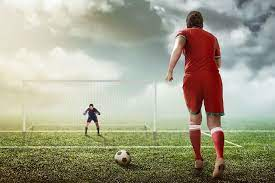
\includegraphics[height=4.5cm]{Q12_1Klausur_Ana_Sto_v2_NachholTermin_01.jpeg}}
\end{center}

\begin{enumerate}[label={\alph*)}] 
  \item Wie viele Elfmeter muss Mannschaft A mindestens schießen, damit sie mit einer Wahrscheinlichkeit von mehr als 99,9\% mindestens einen verwandelt? 
  \item Wie groß muss die Trefferquote der Spieler von Mannschaft B mindestens sein, damit die Wahrscheinlichkeit dafür, dass sie von 5 Elfmetern mindestens einen verwandeln, mindestens 92,0\% beträgt?\\
\\
Als Alternativen zum üblichen Ablauf eines Elfmeterschießens werden die beiden folgenden Verfahren vorgeschlagen. Dabei habe jeder Spieler von B eine Treffer quote von 70\%.

\item Beide Mannschaften schießen je dreimal. Mit welcher Wahrscheinlichkeit endet dieses "Elfmeterduell" unentschieden? 
\item Die Schützen der beiden Mannschaften treten paarweise gegeneinander an: Ein Spieler von A und einer von B schießen je einmal. Liegt danach eine Mannschaft in Führung, endet das Spiel sofort, anderenfalls wird das Verfahren mit dem nächsten Spielerpaar wiederholt. Mit welcher Wahrscheinlichkeit würde bei diesem Vorgehen nach drei angetretenen Paaren noch kein Sieger feststehen?
\end{enumerate}

\vspace{3cm}

\begin{center}
  Viel Erfolg!
\end{center}

%\vspace{2cm}



\end{document}
